\documentclass[letterpaper]{article}
\usepackage{proceed2e}
\usepackage[margin=1in]{geometry}
\usepackage{amsmath,amsthm,epsfig,booktabs}

\newtheorem{lemma}{Lemma}
\newtheorem{theorem}{Theorem}

% Set the typeface to Times Roman
\usepackage{times}

\title{Quotient Normalized Maximum Likelihood Criterion for Learning Bayesian Network Structures}

\author{} % LEAVE BLANK FOR ORIGINAL SUBMISSION.
          % UAI  reviewing is double-blind.

% The author names and affiliations should appear only in the accepted paper.
%
%\author{ {\bf Harry Q.~Bovik\thanks{Footnote for author to give an
%alternate address.}} \\
%Computer Science Dept. \\
%Cranberry University\\
%Pittsburgh, PA 15213 \\
%\And
%{\bf Coauthor}  \\
%Affiliation          \\
%Address \\
%\And
%{\bf Coauthor}   \\
%Affiliation \\
%Address    \\
%(if needed)\\
%}



% Example definitions.
% --------------------
%\def\x{{\mathbf x}}
%\def\L{{\cal L}}

\hyphenation{col-umns}
\hyphenation{Bayes-ian}
\hyphenation{oth-er}

\begin{document}

\maketitle

\begin{abstract}
Learning the dependency structure of a multivariate distribution from
the observational data is an important task since it allows us to
speculate about the underlying causal mechanisms that induce
dependencies. This learning task can be approached as a model
selection problem, but recent studies have revealed that the popular
Bayesian model selection criterion is not satisfactory. We review some
of the information theoretic alternatives and introduce a new one
called a quotient normalized maximum likelihood criterion.
\end{abstract}

\section{INTRODUCTION}
\label{sec:intro}
Bayesian networks~\cite{Pear88} are popular models for presenting
multivariate statistical dependencies that may have been induced by
underlying causal mechanisms.  Techniques for learning the structure
of Bayesian networks from the observational data has therefore been
used for many tasks such as discovering cell signaling pathways from
the protein activity data~\cite{bn4sigpath02}, revealing the business
process structures~\cite{bn4bpmining} from the transaction logs and
modeling brain region connectivity using fMRI
data~\cite{bn4brainconnect}.

Learning the structure of statistical dependencies can be seen as a
model selection task where each model is a different hypothesis about
the conditional dependencies between sets of variables. Traditional
model selection criteria such as the Akaike information
criterion~\cite{Akai73} and the Bayesian information
criterion~\cite{Schw78} have also been used for the task, but recent
comparisons have not been favorable for these criteria in terms of
structural stability and/or predictive
performance~\cite{cosco.pgm08a}.  The most popular criterion has been
the marginal likelihood (usually called BDeu for reasons explained
later), but recent studies~\cite{cosco.uai07,Steck08} have found this
criterion to be very sensitive to hyper parameters and to yield
undesirably complex models for small sample sizes.

The information theoretic normalized maximum likelihood (NML)
criterion~\cite{Shta87,Riss96a} would otherwise be an ideal candidate
for a good criterion.  but its exact calculation is likely to be
prohibitively demanding. In 2008, Silander et al. introduced a
hyper-parameter free, NML inspired criterion called a factorized NML
(fNML)~\cite{cosco.pgm08a} that was shown to yield good predictive
models without sensitivity problems.  However, from the structure
learning point of view, the fNML still sometimes appears to yield
overly complex models. In this paper we introduce another NML related
criterion, a quotient NML (qNML) that yields simpler models without
sacrificing predictive accuracy. Furthermore, unlike the fNML, the
qNML gives equal scores to the structures that encode the same
independence statements. Like other common model selection criteria,
the qNML is also consistent.

We will next briefly introduce Bayesian networks and then review the
BDeu and fNML criteria and introduce the qNML criterion.  We will also
summarize the results for 20 datasets to back up our claim of qNML
yielding parsimonious models with good predictive capabilities.

\section{BAYESIAN NETWORKS}
\label{sec:bns}

Bayesian networks are a general way to describe the dependencies
between the components of an $n$\nobreakdash-dimensional discrete data
vector $X=(X_{1},\ldots,X_{n})$ in which the component $X_{i}$ may
take any of the discrete values in a set $\{1,\ldots,r_{i}\}$.
Despite denoting the values with small integers, the model will treat
the components of $X$ categorical.


\subsection{Likelihood}
\label{ssec:likelihood}

Bayesian network $B=(G,\theta)$ defines a probability distribution for
$X$. The component $G$ defines the structure of the model as a
directed acyclic graph that has exactly one node for each component of
$X$. The structure $G=(G_{1},\ldots,G_{n})$ defines for each
variable/node $X_{i}$ its (possibly empty) parent set $G_{i}$, i.e.,
the nodes from which there are a directed edges to the variable
$X_{i}$.

Given a realization $x$ of $X$, we denote the sub\nobreakdash-vector
of $x$ that consists of the values of the parents of $X_{i}$ in $x$ as
$G_{i}(x)$. It is customary to enumerate all the possible
sub\nobreakdash-vectors $G_{i}(X)$ from $1$ to $q_{i}=\prod_{h\in
  G_{i}}r_{h}.$ In case $G_{i}$ is empty, we define $q_{i}=1$ and
$P(G_{i}(x)=1)=1$ for all vectors $x$.

For each variable $X_{i}$ there is a $q_{i}\times r_{i}$ table
$\theta_{i}$ of parameters whose $j^{\textnormal{th}}$ row and
$k^{\textnormal{th}}$ column defines the conditional probability
$P(X_{i}=k\mid G_{i}(X)=j;\theta)=\theta_{ijk}$.  With structure $G$
and parameters $\theta$, we can now express the likelihood function of
the model as
\begin{equation}
P(x|G,\theta)=\prod_{i=1}^{n}P(x_{i}\mid G_{i}(x);\theta_{i})=\prod_{i=1}^{n}\theta_{iG_{i}(x)x_{i}}.
\end{equation}



\subsection{Bayesian structure learning}

Bayesian learning of Bayesian network structures is based on the
posterior probability $P(G|D,\alpha)$, where $\alpha$ denotes the
hyper\nobreakdash-parameters for the model parameters $\theta$, and
the $D$ is a collection of $N$ $n$\nobreakdash-dimensional i.i.d. data
vectors collected to a $N\times n$ design matrix.  We use structure
$G$ to extend the common matrix indexing notation $D[i,j]$, and allow
more general row selectors.  Notably the notation $D[G_i=j,i]$ is used
to denote those rows of the column $i$ in which the parents $G_i$
contain the value configuration number $j\in\{1,\ldots,q_i\}$.

It is common to assume the uniform prior for structures, in which case
the objective function for structure learning is reduced to the
marginal likelihood $P(D|G,\alpha)$.  If the model parameters
$\theta_{ij}$ are further assumed to be independently Dirichlet
distributed only depending on $i$ and $G_{i}$ and the data $D$ is
assumed to have no missing values, the marginal likelihood can be
decomposed as
\begin{eqnarray}
\label{eqn:bayesmix}
P(D|G,\alpha) & = & \prod_{i=1}^{n}\prod_{j=1}^{q_i}\int
P(D[G_i=j,i]|\alpha)\\ & = & \prod_{i=1}^{n}\prod_{j=1}^{q_i}\int
P([G_i=j,i]|\theta)P(\theta|\alpha) d\theta.\nonumber
\end{eqnarray}
In coding terms this means that each data column $D[\cdot,i]$ is first partitioned based on the
values in columns $G_i$, and each part is then coded using a Bayesian mixture that can be expressed
in a closed form~\cite{Bunt91, Heck95}.

\subsection {Problems, solutions and problems}

Finding the satisfactory Dirichlet hyperparameters for the Bayesian
mixture above has, however, turned out to be problematic. Early on,
one of the desiderata for a good model selection criterion was that it
would yield equal scores for essentially equivalent
models~\cite{Verm90}.  For example, the score for the structure
$X_1\rightarrow X_2$ should be the same as the score for the model
$X_2 \rightarrow X_1$ since they both correspond to the hypothesis
that variables $X_1$ and $X_2$ are statistically dependent on each
other.  It can be shown~\cite{Heck95} that to achieve this, not all
the hyperparameters $\alpha$ are possible and for practical reasons
Buntine~\cite{Bunt91} suggested a so called BDeu score with just one
hyperparameter $\alpha\in R_{++}$ so that $\theta_{ij\cdot}\sim
Dir(\frac{\alpha}{q_i r_i},\ldots,\frac{\alpha}{q_i r_i})$.  However,
it soon turned out that BDeu score was very sensitive to the selection
of this hyperparameter~\cite{cosco.uai07} and that for small sample
sizes this method detects spurious correlations~\cite{Steck08} leading
to models with suspiciously many parameters.

A natural solution to avoid parameter sensitivity of BDeu would be to
use a normalized maximum likelihood (NML)
criterion~\cite{Shta87,Riss96a}, i.e., to find the structure $G$ that
maximizes
\begin{equation}
P_{NML}(D;G)=\frac{P(D|\hat\theta(D;G))}{\sum_{D'}{P(D'|\hat\theta(D';G))}},
\end{equation}
where $\hat\theta$ denotes the (easy to find) maximum likelihood
parameters and the sum in the denominator goes over all the possible
$N\times n$ data matrices. While it is easy to see that this criterion
satisfies the requirement of giving equal scores to equal structures,
the normalizing constant renders the computation
infeasible. Consequently, Silander et al.~\cite{cosco.pgm08a}
suggested solving the parameter sensitivity problem by adopting the
NML-code to the column partitions, i.e., changing the Bayesian mixture
in equation~(\ref{eqn:bayesmix}) to
\begin{equation}
P^1_{NML}(D[G_i=j,i];G)=\frac{P(D|\hat\theta(D[G_i=j,i];G))}{\sum_{D'}{P(D';\hat\theta(D'|G))}},
\end{equation}
where $D'\in{\{1,\ldots,r_i\}}^{|D[G_i=j,i]|}$.  The logarithm of the
denominator is often called a regret, since it indicates the extra
code length needed compared to the code length obtained using the (a
priori unknown) maximum likelihood parameters. The regret for
$P^1_{NML}$ depends only on the length $N$ of the categorical data
vector with $r$ different categorical values.  While the naive
computation of the regret is still prohibitive, it can be approximated
efficiently using a so called Szpankowski
approximation~\cite{cosco.aistat03}:
\begin{eqnarray}
\label{eqn:szp}
\lefteqn{reg(N,r) \approx \frac{\sqrt{2} r \Gamma{\left(\frac{r}{2} \right)}}
                               {3 \sqrt{N} \Gamma{\left(\frac{r-1}{2}  \right)}}} \\
&&+ \left(\frac{r-1}{2}\right) \log{\left (\frac{N}{2} \right )}
- \log \Gamma{\left(\frac{r}{2} \right)} + \frac{1}{2} \log{\left (\pi \right )}\nonumber\\
&&- \frac{r^{2} \Gamma^{2}{\left(\frac{r }{2} \right)}}
         {9N \Gamma^{2}{\left(\frac{r-1}{2}\right)}}
+ \frac{2r^3-3r^2-2r+3}{36N}\nonumber.
\end{eqnarray}
fNML solves the parameter sensitivity problem and yields predictive
models superior to BDeu.  However, the criterion does not satisfy the
property of giving the same score for the models that correspond to
the same dependence statements. Furthermore, the learned structures
still sometimes appear surprisingly complicated.
 
\section{QUOTIENT NML SCORE}

We will now introduce a quotient normalized maximum likelihood (qNML)
criterion for learning Bayesian network structures.  While equally
efficient to compute than BDeu and fNML, it is free from
hyperparameters, and it can be proven to give equal scores to
equivalent models. Furthermore, it coincides with the actual NML score
for exponentially many models. In our empirical tests it produces
models featuring good predictive performance with significantly
simpler structures than BDeu and fNML.

Like BDeu and fNML, qNML can be expressed as a product of $n$ terms,
one for each variable, but unlike the other two, it is not based on
further partitioning the corresponding data column
\begin{eqnarray}
s^{qNML}(D;G) & := & \sum_{i=1}^n s^{qNML}_i(D;G)\\
& := & \sum_{i=1}^n \log \frac{P^1_{NML}(D[\cdot,(i,G_i)];G)}
                             {P^1_{NML}(D[\cdot,G_i];G)}.\nonumber
\end{eqnarray}
The trick here is to model a subset of columns as though there were no
conditional independencies among the corresponding variables $S
\subset X$.  In this case, we can collapse the $\prod_{X_i\in S} r_i$
value configurations and consider them as values of a single variable
with $\prod_{X_i\in S} r_i$ different values which can then be modeled
with a one-dimensional $P^1_{NML}$ code.  The $s^{qNML}$ does not
necessarily define a distribution for $D$, but it is easy to verify
that it coincides with the $P_{NML}(D;G)$ for all the networks that
are composed of fully connected components.  The number of such
networks equals the number of nonempty partitions of a set of $n$
elements, i.e., the $n^\text{th}$ Bell number.

\subsection {qNML is score equivalent}

The qNML yields equal scores for network structures that encode same
sets of independencies. Verma and Pearl~\cite{Verm90} showed that the
equivalent networks are exactly those who a) are same when directed
arcs are substitued by undirected ones and b) who have same
V-structures, i.e.  the variable triplets $(A,B,C)$ where both $A$ and
$B$ are parents of $C$, but there is no arc between $A$ and $B$ (in
neither direction).  Later, Chickering~\cite{Chick95} showed that all
the equivalent network structures, and only them, can be reached from
each other by reversing, one by one, so called covered arcs, i.e. the
arcs from node $A$ to $B$, for which $B$'s parents other than $A$ are
exactly the $A$'s parents ($G_B=\{A\}\cup G_A$).

We will next state this as a
theorem and sketch a proof for it. A more detailed proof appears in the
suplementary material.
\begin{theorem}
  \label{thm:scoreqv}
  Let $G$ and $G'$ be two Bayesian network structures that differ only
  by a single covered arc reversal, i.e., the arc from $A$ to $B$ in $G$
  has been reversed in $G'$ to point from $B$ to $A$, then
  $$s^{qNML}(D;G)=s^{qNML}(D;G').$$
\end{theorem}
\begin{proof}
  Now the scores for structures can be decomposed as the
  $s^{qNML}(D;G)=\sum_{i=1}^{n}s_i^{qNML}(D;G)$ and
  $s^{qNML}(D;G')=\sum_{i=1}^{n}s_i^{qNML}(D;G')$.  Since only the
  terms corresponding to the variables $A$ and $B$ in these sums are
  different, it is enough to show that sum of these two terms are
  equal for $G$ and $G'$. Since we can assume the data to be fixed we
  lighten up the notations and write
  $P^1_{NML}(i,G_i) := P^1_{NML}(D[\cdot,(i,G_i)];G)$ and
  $P^1_{NML}(G_i)   := P^1_{NML}(D[\cdot,G_i];G)$.
  \begin{eqnarray}
    \lefteqn{s_A^{qNML}(D;G)+s_B^{qNML}(D;G)} \nonumber\\
    && =\log\frac{P^1_{NML}(A,G_{A})}{P^1_{NML}(G_{A})}
            \frac{P^1_{NML}(B,G_{B})}{P^1_{NML}(G_{B})}\nonumber\\
    && =\log 1\cdot\frac{P^1_{NML}(B,G_{B})}{P^1_{NML}(G_{A})}\nonumber\\
    && =\log \frac{P^1_{NML}(B,G'_{B})}{P^1_{NML}(G'_{A})}
             \frac{P^1_{NML}(A,G'_{A})}{P^1_{NML}(G'_{B})}\nonumber\\
 && =s_A^{qNML}(D;G')+s_B^{qNML}(D;G'),\nonumber
\end{eqnarray}
  due to equations
  $\{A\}\cup G_A  = G_B$,
  $\{B\}\cup G'_B = G'_A$,
  $\{B\}\cup G_B  = \{A\} \cup G'_A$,
  and $G_A        = G'_B$.
\end{proof}

\subsection{qNML is consistent}


\subsection {On implementation}

Collapsing many variables into a single one causes $r$ in the
equation~(\ref{eqn:szp}) to be exponentially large (in our experiments
around $2^{20}$).  This causes the $\Gamma^2$ terms to grow very large
calling for care when computing the ratios of such huge numbers. More
specifically, scoring the $i^\text{th}$ data column, i.e., computing
$s^{qNML}_i$, requires the difference $dreg(N,q_i,r_i)=reg(N,q_i) -
reg(N,r_i q_i)$, where $q$ denotes the number of values in the
collapsed parent variable.  A numerically stable approximation is:
\begin{eqnarray}
\lefteqn{dreg(N,q,r)\approx\frac{1-r^2}{18 N} q^{2}} \\
&&+ \frac{\left(q - 1\right) \sqrt{4 q - 2} + \left(1 - q r\right) \sqrt{4 q r - 2}}{6 \sqrt{N}} \nonumber\\
&&+\frac{q\left(3 N \left(r \log{r}  - \left(r - 1\right) \left(\log{N} + 1\right)\right) + r\right)}{6 N} \nonumber\\
&&+ \frac{1}{12}(\log{(r+\frac{1-r}{q+1})}- 7\log{r}).\nonumber
\end{eqnarray}

\section{EXPERIMENTAL RESULTS}

To empirically compare the model selection criteria we took 20 UCI
data sets~\cite{Lichman:2013} and run 1000 train and test experiments
for 20 different sample sizes for all of them. The training was
conducted using a dynamic programming based exact structure
learning\cite{cosco.uai06} which limited the number $n$ of variables
to less than 20.

Figure~\ref{fig:bcmean} shows an example of the behavior of the
studied selection criteria.  For small sample sizes fNML and qNML
yield equally accurate predictions while BDeu requires more samples to
obtain competitive performance. The curves are mean curves from 1000
independent train and test splits.

\begin{figure}
\centering
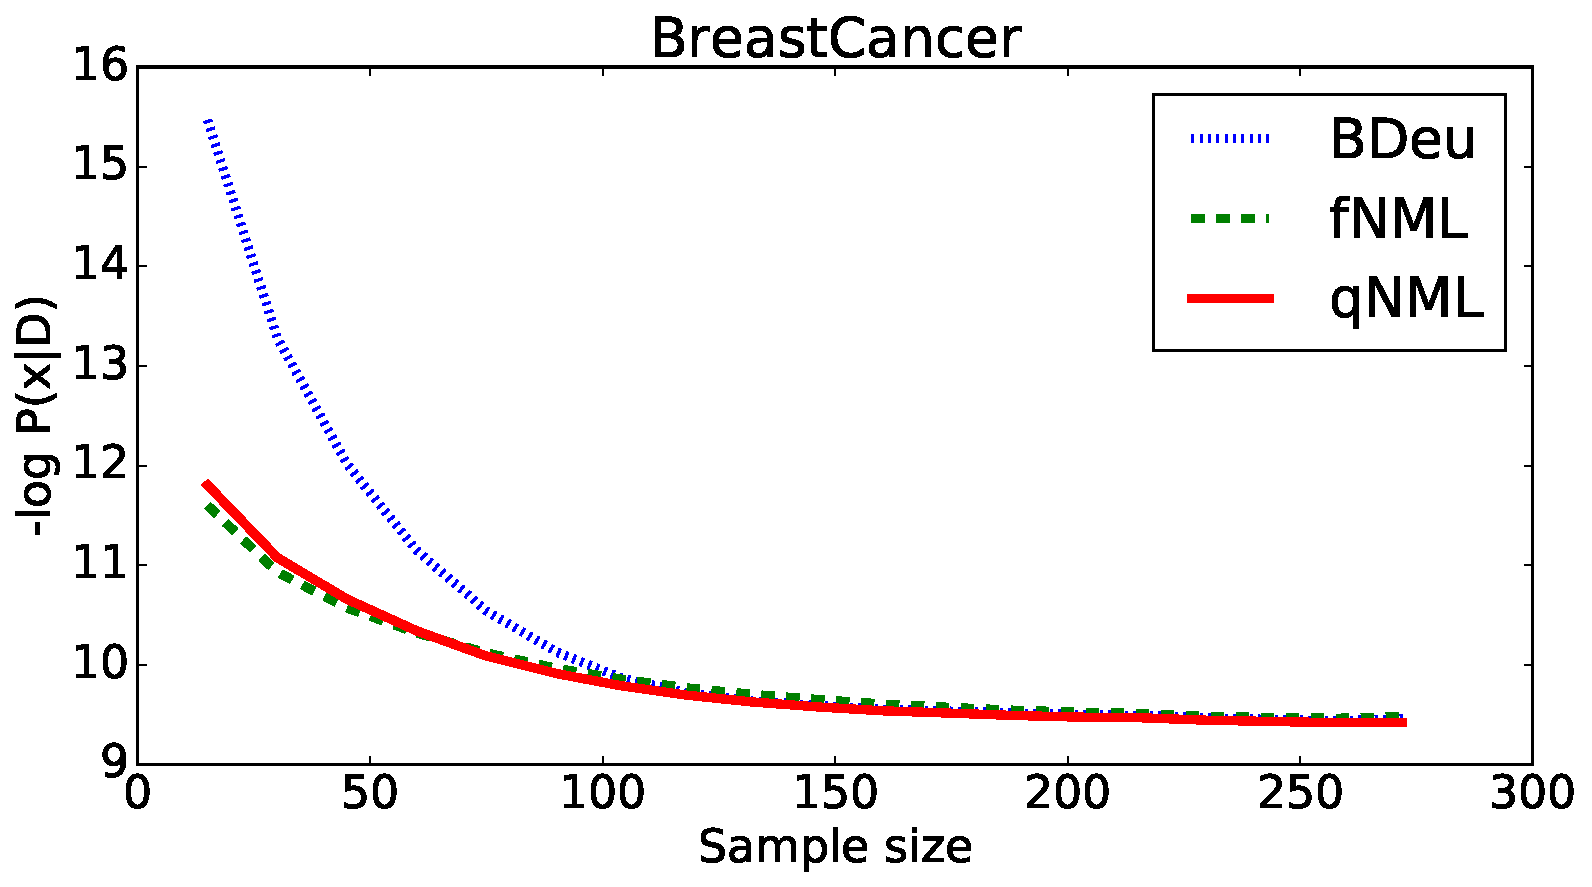
\includegraphics[width=8cm,height=5cm]{breast_cancer_mean.pdf}
\caption{Predictive log-loss in a breast cancer data as a function of
  sample size for different model selection criteria.}
\label{fig:bcmean}
\end{figure}

Figure~\ref{fig:bcnpmean} shows how fNML still sometimes behaves
strangely in terms of model complexity here measured by the number of
parameters in the model.  qNML, instead, appears to yield more
parsimonious models.

\begin{figure}
\centering
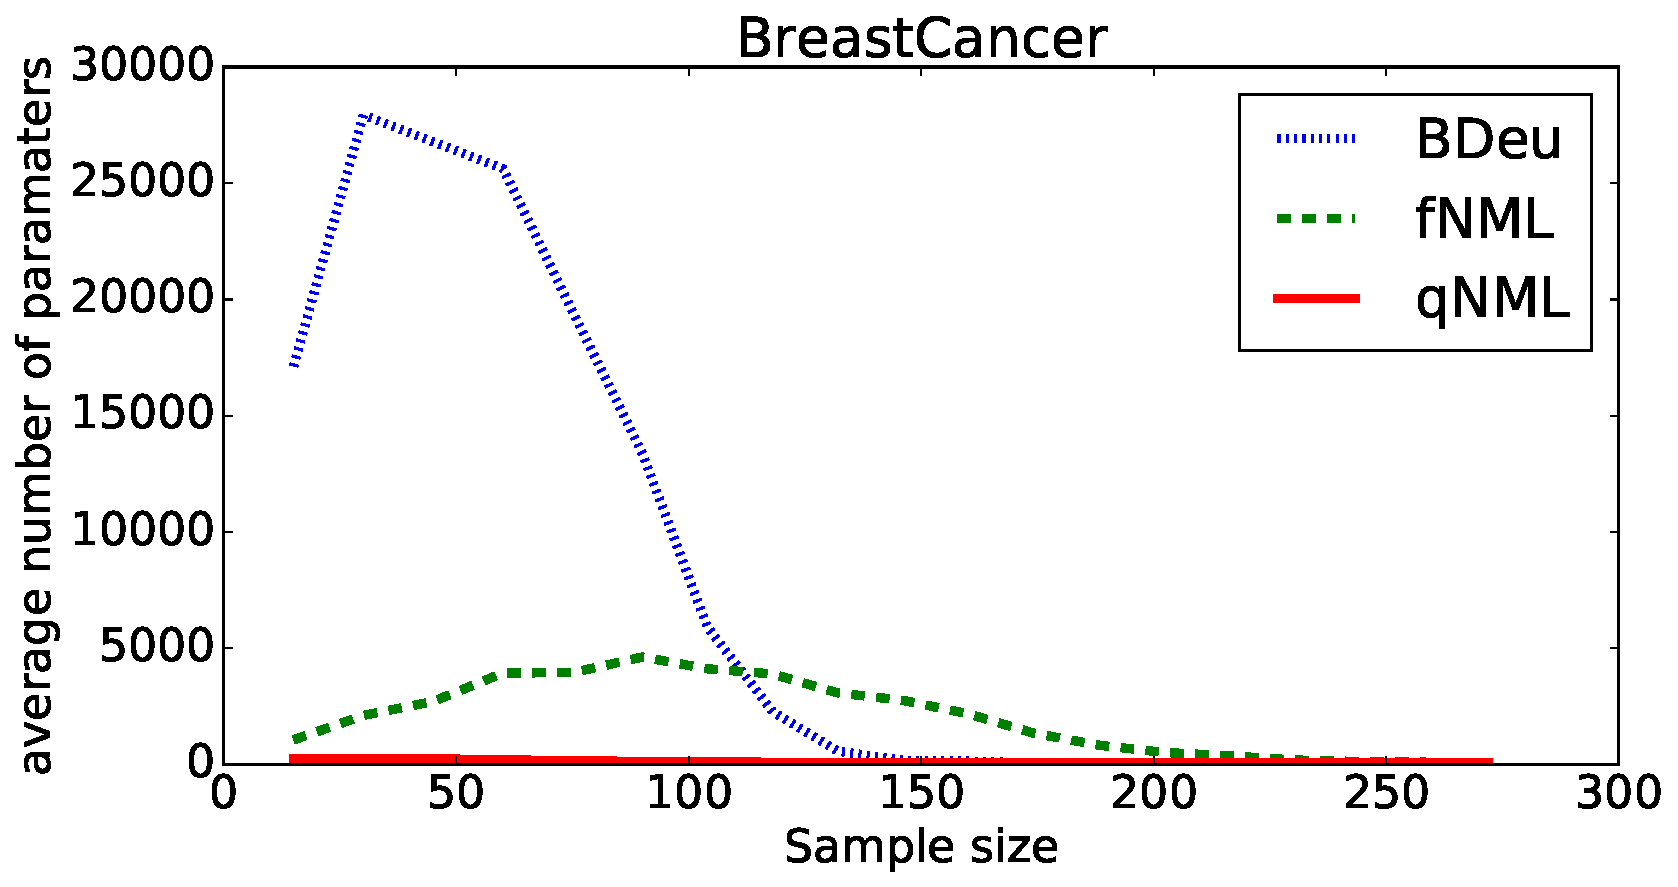
\includegraphics[width=8cm,height=5cm]{breast_cancer_np_mean.pdf}
\caption{Number of parameters in a breast cancer model as a function
  of sample size for different model selection criteria.}
\label{fig:bcnpmean}
\end{figure}

\begin{table}
\centering
\begin{tabular}{crrrr}
\toprule
           Data &     N &   BDeu &            fNML &            qNML \\
\midrule
           Iris &    16 &   3.59 &            3.47 &   \textbf{3.43} \\
  PostOperative &    20 &  10.24 &   \textbf{8.27} &            8.32 \\
           Wine &    27 &  18.11 &           12.68 &  \textbf{12.51} \\
 HeartHungarian &    45 &  10.15 &            9.10 &   \textbf{8.90} \\
   BreastCancer &    45 &  12.01 &  \textbf{10.57} &           10.66 \\
 HeartCleveland &    48 &  16.36 &           12.81 &  \textbf{12.54} \\
          Ecoli &    51 &   5.77 &   \textbf{5.30} &            5.37 \\
          Liver &    54 &   4.07 &            3.97 &   \textbf{3.91} \\
          Glass &    55 &   7.16 &   \textbf{6.22} &            6.28 \\
        Thyroid &    55 &   2.83 &   \textbf{2.75} &            2.77 \\
   HeartStatlog &    56 &  14.15 &           11.92 &  \textbf{11.60} \\
      TicTacToe &    96 &  10.99 &  \textbf{10.73} &           11.05 \\
        Balance &    96 &   7.48 &   \textbf{7.39} &            7.78 \\
    BcWisconsin &   105 &   5.81 &            5.12 &   \textbf{5.08} \\
       Diabetes &   117 &   4.95 &            4.95 &   \textbf{4.89} \\
          Yeast &   225 &   5.54 &   \textbf{5.40} &            5.42 \\
        Abalone &   418 &   3.93 &   \textbf{3.88} &            3.96 \\
     PageBlocks &   548 &   2.36 &   \textbf{2.32} &            2.38 \\
        Shuttle &  2900 &   1.70 &   \textbf{1.69} &            1.72 \\
          Adult &  4885 &  10.22 &  \textbf{10.08} &           10.12 \\
\bottomrule
\end{tabular}
\caption{Predictive log losses for small sample sizes for different model selection criteria in 20 different datasets.}
\label{tbl:preds}
	\end{table}

Table~\ref{tbl:preds} features predictive losses for the small sample
sizes.  (The results for large sample sizes converge for all sensible
criteria.)  As we can see, fNML still usually (12/20) performs best
but qNML is not much worse while BDeu may sometimes perform much
worse.

Looking at the number of parameters for the same datasets and sample
sizes (Table~\ref{tbl:nofparams}) reveals that qNML usually (18/20)
yields simplest models, and sometimes, like in the BreastCancer data,
the differences are of orders of magnitude.

\begin{table}
\centering
\begin{tabular}{crrrr}
\toprule
           Data &     N &          BDeu &  fNML &          qNML \\
\midrule
           Iris &    16 &            36 &    33 &   \textbf{28} \\
  PostOperative &    20 &          1304 &   464 &  \textbf{115} \\
           Wine &    27 &         11559 &   780 &  \textbf{214} \\
 HeartHungarian &    45 &          4706 &   838 &  \textbf{100} \\
   BreastCancer &    45 &         26774 &  2710 &  \textbf{246} \\
 HeartCleveland &    48 &         29346 &  1407 &  \textbf{204} \\
          Ecoli &    51 &           113 &   167 &   \textbf{80} \\
          Liver &    54 &            40 &    60 &   \textbf{24} \\
          Glass &    55 &          1488 &   572 &  \textbf{100} \\
        Thyroid &    55 &            37 &    70 &   \textbf{28} \\
   HeartStatlog &    56 &         18414 &  1099 &  \textbf{159} \\
      TicTacToe &    96 &         13645 &  2438 &  \textbf{696} \\
        Balance &    96 &   \textbf{20} &   237 &           168 \\
    BcWisconsin &   105 &          5921 &   816 &   \textbf{88} \\
       Diabetes &   117 &            35 &   216 &   \textbf{34} \\
          Yeast &   225 &   \textbf{78} &   307 &            80 \\
        Abalone &   418 &            90 &   156 &   \textbf{62} \\
     PageBlocks &   548 &           699 &   377 &   \textbf{56} \\
        Shuttle &  2900 &           380 &   594 &  \textbf{111} \\
          Adult &  4885 &  \textbf{599} &  1431 &           876 \\
\bottomrule
\end{tabular}
\caption{Number of model parameters for small sample sizes for different model selection criteria in 20 different datasets.}
\label{tbl:nofparams}
\end{table}

\section{CONCLUSION}

We have presented qNML, a new model selection criterion for learning
structures of Bayesian networks.  While being competitive in
predictive terms, it often yields significantly simpler models than
other common model selection criteria.  The computational cost of qNML
equals the cost of earlier criteria.  The criterion also gives equal
scores for models that encode same independence hypotheses about the
joint probability distribution.  qNML also coincides with NML
criterion for exponentially many models.

\subsubsection*{Acknowledgements}

Use unnumbered third level headings for the acknowledgements title.
All acknowledgements go at the end of the paper.


%%\subsubsection*{References}

\bibliographystyle{apalike}
\bibliography{cosco}

\end{document}
